\documentclass{article}

\usepackage{cite}
\usepackage{float}
\usepackage{graphicx}

\linespread{1.3}

\title{Telemetry-based Optimisation for User Training in Racing Simulators}
\author{Francois Buhagiar}
\date{2015}

\begin{document}

\pagenumbering{roman} 

\maketitle

\pagenumbering{arabic} 
\setcounter{page}{1}

\begin{abstract}
\end{abstract}

\newpage
\section{Introduction}

\newpage
\section{Literature Review}

In the following section an explanation will be given for the ground work on which this final year project is based upon. The areas which will be covered include video games and serious games focusing on the differences between the two, which will be used to introduce the idea of using serious games as a training mechanism. Motorsport circuit car racing will also be discussed, describing what it involves from a formal point of view by defining the tasks which a racing driver is required to carry out in order to get a good lap time. 

\subsection{Video games and Serious Games}

Baranowski and colleagues defined games as “a physical or mental contest with a goal or objective, played according to a framework, or rule, that determines what a player can or cannot do inside a game world” the definition covers the setup of a game, while  "a physical or mental contest, played according to specific rules, with the goal of amusing or rewarding the participant"\cite{yuserious}.

Video games are built on top of these core values with the difference of having the game world confined into some sort of digital media. According to historians video games started with William Higinbotham who created a tennis game to be played on a television set\cite{stanton2015brief}. From the early days of video games, their main aim was always to provide some degree of entertainment. The entertainment value is achieved in various ways depending on gaming platform, game genre and the audience the video game is targeted to. According to Electronic Arts chief creative officer at the time, modern video games are simply made up of three fundamental components, story, art and software\cite{zyda2005visual}.

The definition of serious games has been redefined multiple times. The first formal definition appears to have been introduced by Abt in his book from 1970 which stated a serious game to be simulations and games to improve eduction\cite{abt1970}. Several years later, a white paper written by Sawyer in 2002 proposed an updated definition to be based on the idea of connecting a serious purpose to knowledge and technologies from the video game industry\cite{michael2005serious}. Moving on to nowadays definitions such as the ones from Chen and Michael in 2005\cite{michael2005serious} and from Zyda also in 2005\cite{zyda2005visual} seem to stem from Swayer's influence. The boundaries of serious games are debated, mostly due to the fact that serious game attract multiple domains making it hard to come up with a common boundary. However, the common denominator across all domains seems to be "Serious Game designers use people's interest in video games to capture their attention for a variety of purposes that go beyond pure entertainmnet"\cite{djaouti2011classifying}.

From the above one stands to reason the main contrast between video games and serious games involve the use of pedagogy activities that aim to educate or instruct knowledge or skill\cite{zyda2005visual} in serious games. These activities are given preference over entertainment value, hence the amusement aspect which are custom to video games might not be found at all in a serious game\cite{zyda2005visual}. 

\subsection{Consumer sim racing games as a serious game}

Sim racing games such as Asseto Corsa and Project Cars which are consumer available of the shelf, provide a sim racing experience within the average cost of other consumer games. The aim of sim racing games is to replicate real life cars, race car dynamics and track locations with the aim of providing entertainment and amusement to the player. The challenge aspect is achieved by paring the user against other AI players, multiplayer online races played against other human players, or sometimes against ones self. These points make racing games fit the previous definition of what a video game is however, fail to meet the requirements of a serious game, they miss the pedagogy activities. Most of the modern sim racing games do aid the player to improve by means of implementing aids. Such aids might include showing the racing line to which the player is expected to drive on, while also showing the braking and acceleration points. Other aids include anti lock brakes, traction control and stability control. The problem with their implementation is, the fact of them being implemented in a passive way. With the exception of the racing line, the player is not told when and what is being done wrong. The result is, users having to figure their own mistakes out by means of practicing without any guidance or feedback from with the game. This final year project aims to implement a module which is plugged into an off the shelf racing simulator which. This module trains users by letting them know what is being done wrong, when it's being done wrong and most importantly how to avoid making the same mistake.

[Show image of racing line red / green ?]
[In appendix, we might need to explain what ABS, TCS AND STC are]

\subsection{Serious games as a training mechanism}

As mentioned, serious games focus on the pedagogy activities 

\subsection{Circuit motorsport racing, getting near the optimal lap time}

"A situation in which individuals or groups compete to be first to achieve a particular objective." is what the Oxford dictionary defines a race to be. This can be more specifically defined to describe circuit motorsport races, in which motorised vehicles go round a course called a circuit. Each racing discipline or series has it's own rules however, at the core all disciplines participants aim to complete a full lap of the circuit in the least amount of time. Some disciplines focus on achieving one fast lap, such as time trials, while others focus on achieving the least amount of time across a fixed amount of laps, such as FIA's Formula 1 series.

Moving over to defining the problem which a race driver faces, that of "figure out how to go round a piece of asphalt in the minimum amount of time"\cite{GoingFaster}. In order to do so, the race driver needs to develop techniques which aid in controlling the vehicle which is being raced. Such technique is that of mastering the race line, which is considered the the fundamental skill a race driver must understand and master before moving on to anything else\cite{GoingFaster}. The best path through a corner is said to be one which takes the least time while keeping the higher average speed\cite{beckman1991physics}. The trickiest part of the racing line to master is that of a corner, below a basic understanding of the racing line is given for corner.

\begin{figure}
	\centering
	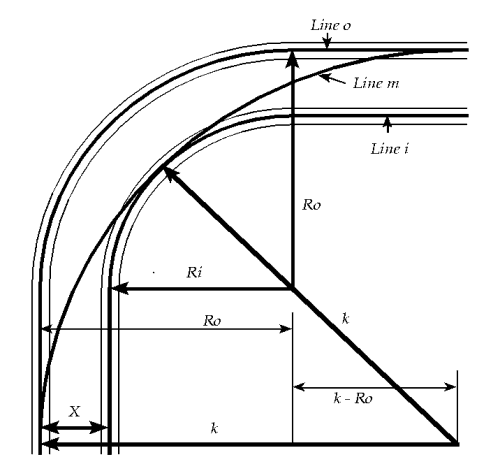
\includegraphics[height=5cm]{Racing_Corner.png}
	\caption{Multiple possible racing lines round a corner}
	\label{fig:Racing_Corner}
\end{figure}

In Figure~\ref{fig:Racing_Corner} actually represents a family of corners with any constant width, any radius, and short straights before and after. First, we go through the entire analysis with a particular corner of 75 foot radius and 30 foot width, then we end up with times for corners of various radii and widths. 
Let us define the following parameters:
	r = radius of corner centre line = 75 feet
	W = width of course = 30 feet
	ro = radius of outer edge = r + ½W = 90 feet
	ri = radius of inner edge = r - ½W = 60 feet
Now, when we drive this corner, we must keep the tyres on the course, otherwise we get a lot of cone penalties (or go into the weeds). It is easiest (though not so realistic) to do the analysis considering the path of the centre of gravity of the car rather than the paths of each wheel. So, we define an effective course, narrower than the real course, down
which we may drive the centre of the car.
	w = width of car = 6 feet
	Ro = effective outer radius = ro - ½w = 87 feet
	Ri = effective inner radius = ri + ½w = 63 feet
	X = effective width of course = W - w = 24 feet

-----------------
Techniques vary depending on the vehicle, circuit and weather, for the purpose of keeping things simple and focused this thesis will focus on techniques required on tarmac racing in dry weather conditions. A discipline a using a vehicle which isn't hard to control which in turns also the driver the focus on getting the core techniques right.

This thesis will focus on training an individual to achieve good laps times while also being consistent. This will be carried out by lookin

What is the task of a racing driver ?


\subsection{User study}
Maybe write something about how the approach the user study? Maybe find a Literature on how to ask user for their feedback which will be used for the survey after using the system.

\newpage
\section{Methodology}

\newpage
\bibliography{citeations}{}
\bibliographystyle{plain}

\end{document}